\section{Example Single Water Tank RabbitMQ}\label{sec:example-watertank}
The example in this section concerns a water tank with constant inflow and a
drain valve as depicted in \cref{fig:water-tank-picture}. The water level should
stay within a parameterised minimum and maximum water level. This is a brief
description, please see~\cite{INTOCPSD3.6} for additional information on
the models and co-simulation. Furthermore, historical data is passed in through
RabbitMQ FMU. \textbf{The entire example including a docker-compose file for
  starting a local RabbitMQ Node is available at \url{https://github.com/INTO-CPS-Association/example-single_watertank_rabbitmq}.}
\begin{figure}[!htb]
  \centering
  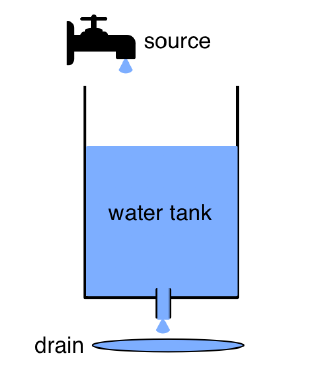
\includegraphics[]{figures/water-tank-picture.png}
  \caption{Water Tank}
  \label{fig:water-tank-picture}
\end{figure}

The example setup is shown in \cref{fig:rabbitmq-example} and consists of:
\begin{description}
  \item[Maestro] FMI Co-Simulation Engine
    \item[Tank FMU] Models the physical part of the water tank and outputs the
    water level within the tank. It receives the state of the drain valve as input.
    \item[Controller FMU] Models the controller of the drain valve. It outputs
    the state of the drain valve and receives the water level as input.
    Furthermore, it has the minimum water level and maximum water level as
    parameters
    \item[RabbitMQ Server] runs a RabbitMQ node.
  \item[Data] Contains historical water level data.
  \item[Python] Reads the data file and inputs it to RabbitMQ.
  \item[RabbitMQ FMU] Subscribes to RabbitMQ data.
    \item[Diff FMU] Only part of the co-simulation for technical issues related to plotting outputs.
\end{description}
\begin{figure}[!htb]
  \centering
  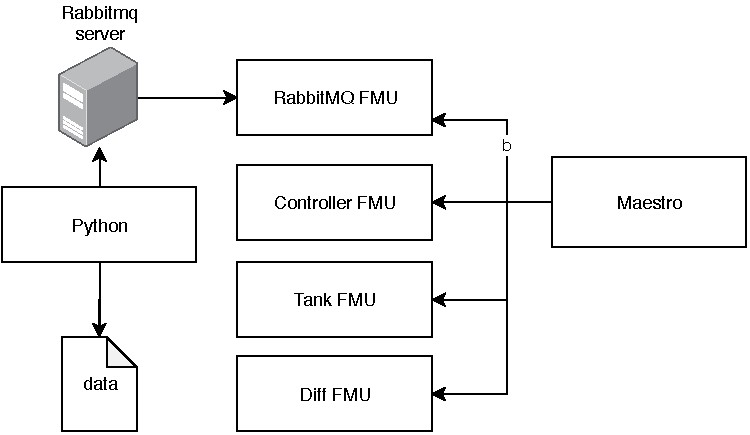
\includegraphics[]{figures/rabbitmq-example.pdf}
  \caption{Water Tank}
  \label{fig:rabbitmq-example}
\end{figure}

The result of executing the co-simulation is shown in \cref{fig:modelled-tank-vs-rabbitmq-fmu-tank}. The discrepancies
between the Tank FMU output and the RabbitMQ FMU output is related to
floating-point imprecision\footnote{See \cite{Cremona2019} for more information on floating-point
  imprecision in relation to FMI.}. By changing the \texttt{precision} as described in
\cref{subsec:cqa} there are no discrepancies.
\begin{figure}[!htb]
  \centering
  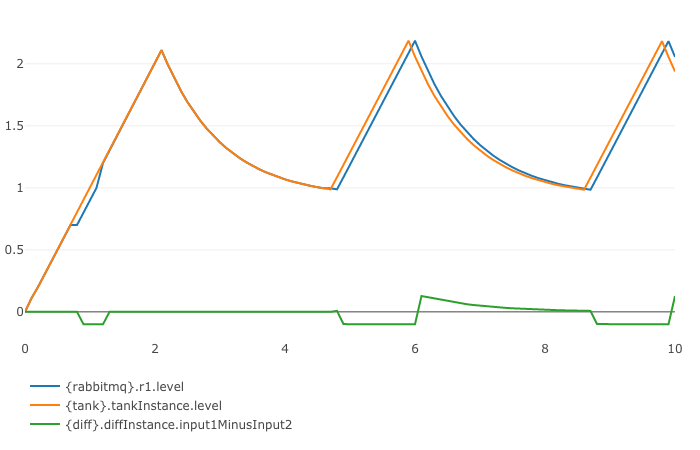
\includegraphics[width=\textwidth]{figures/lfmqtt.png}
  \caption{Modeled tank output and RabbitMQ FMU tank output}
  \label{fig:modelled-tank-vs-rabbitmq-fmu-tank}
\end{figure}





%%% Local Variables:
%%% mode: latex
%%% TeX-master: "../rabbitmq-fmu"
%%% End:
